\section{Backend - Raspberry Pi}

Backend systému beží na jednodoskovom počítači Raspberry Pi 4B (verejná IP adresa
\texttt{147.175.105.185}) a tvorí centrálnu komunikačnú a dátovú vrstvu celého IoT
riešenia. Zodpovedá za príjem dát z ESP32, ich archiváciu, distribúciu do frontendu
v reálnom čase a odosielanie príkazov späť na mikrokontrolér.

\subsection{Flask + SocketIO}

Webový server je implementovaný pomocou mikroframeworku \textbf{Flask} pomocou
knižnice \textbf{Flask-SocketIO}. Flask zabezpečuje klasické HTTP endpointy, zatiaľ čo SocketIO umožňuje obojsmernú
komunikáciu v reálnom čase medzi serverom a prehliadačom bez nutnosti opakovania
HTTP požiadaviek.

Server počúva na porte \texttt{5000} a je nakonfigurovaný pre viacvláknový asynchrónny
režim ..
(\texttt{async\_mode='threading'}), čo umožňuje súbežné spracovanie MQTT správ
a WebSocket udalostí.

Kľúčové SocketIO udalosti:
\begin{itemize}
  \item \texttt{command} -- príjem príkazov z frontendu (OPEN, START, STOP, CLOSE,
        MODE1/2/3, SET\_PID, HEATER\_PULSE),
  \item \texttt{data} -- vysielanie nameraných hodnôt do všetkých pripojených klientov,
  \item \texttt{system\_status} -- informácia o stave systému (inicializovaný / beží),
  \item \texttt{pid\_updated} / \texttt{pid\_error} -- potvrdenie alebo odmietnutie
        zmeny PID parametrov,
  \item \texttt{heater\_status} -- informácia o stave simulácie poruchy.
\end{itemize}

Autentifikácia je riešená pomocou \textbf{Flask session} s dvoma rolami:
\textit{operator} (plný prístup – ovládanie aj sledovanie) a \textit{spectator}
(iba sledovanie). Prístup k chráneným endpointom je vynucovaný dekorátorom
\texttt{login\_required}.

\subsection{MQTT broker (Mosquitto)}

Komunikácia medzi ESP32 a Raspberry Pi prebieha prostredníctvom protokolu \textbf{MQTT}.
Na Raspberry Pi beží broker \textbf{Mosquitto}, na ktorý sa ESP32 pripája cez WiFi.
Flask backend si udržiava vlastného MQTT klienta (\texttt{paho-mqtt}), ktorý je prihlásený
na odber témy \texttt{peltier/data} a zároveň publikuje príkazy na tému
\texttt{peltier/cmd}.

Formát správy z ESP32 je textový CSV riadok:
\begin{verbatim}
<time_ms>,<temp_C>,<tec_pwm>,<pump_pwm>,<mode>
\end{verbatim}
Správy začínajúce znakom \texttt{\#} a riadky s menej ako 5 poľami sú ignorované.
Hodnoty teploty pod \texttt{-100\,°C} sú považované za chybu senzora a tiež sa zahadzujú.

Príkazy posielané na ESP32:
\begin{itemize}
  \item \texttt{STABILIZE} -- ustálenie systému po štarte (TEC 25\,\%, pumpa 50\,\%),
  \item \texttt{MANUAL:tec:pump} -- manuálne nastavenie PWM hodnôt (Mód 1),
  \item \texttt{PID\_TEC} -- spustenie PID regulácie TEC (Mód 2),
  \item \texttt{PID} -- spustenie PID regulácie pumpy (Mód 3),
  \item \texttt{HEATER\_ON / HEATER\_OFF} -- zapnutie/vypnutie ohrievača (simulácia poruchy),
  \item \texttt{SET\_SP / SET\_KP / SET\_KI / SET\_KD} -- aktualizácia parametrov regulácie,
  \item \texttt{STOP} -- zastavenie všetkých výstupov.
\end{itemize}

\subsection{SQL databáza}

Každá prijatá meracia správa je uložená do \textbf{SQLite} databázy
(\texttt{peltier.db}) prostredníctvom ORM knižnice \textbf{Flask-SQLAlchemy}.
Databáza je jediným zdrojom pravdy (\textit{single source of truth}) pre historické dáta.

Tabuľka \texttt{Measurement} obsahuje nasledujúce stĺpce:

\begin{table}[H]
\centering
\begin{tabular}{|l|l|l|}
\hline
\textbf{Stĺpec} & \textbf{Typ} & \textbf{Popis} \\
\hline
\texttt{id}       & INTEGER  & Primárny kľúč (auto-increment) \\
\texttt{time\_ms} & INTEGER  & Čas od štartu merania v milisekundách \\
\texttt{temp\_C}  & FLOAT    & Teplota kvapaliny v °C \\
\texttt{tec\_pwm} & INTEGER  & PWM hodnota TEC (0--255) \\
\texttt{pump\_pwm}& INTEGER  & PWM hodnota pumpy (0--255) \\
\texttt{mode}     & TEXT     & Aktívny mód (MODE1 / MODE2 / MODE3 / STOP) \\
\texttt{setpoint} & FLOAT    & Žiadaná hodnota teploty v °C \\
\texttt{created}  & DATETIME & Čas záznamu (UTC) \\
\hline
\end{tabular}
\caption{Štruktúra tabuľky \texttt{Measurement} v SQLite databáze}
\end{table}

REST endpoint \texttt{/api/history} vracia záznamy zoradené chronologicky s možnosťou
filtrovania podľa časového rozsahu (parameter \texttt{hours}) -- tieto dáta sa
načítavajú pri inicializácii grafu na dashboarde.

\subsection{CSV + JSON archivácia}

Backend umožňuje export databázy meraní vo formátoch \textbf{CSV} a \textbf{JSON}
prostredníctvom HTTP endpointov \texttt{/api/download/csv} a \texttt{/api/download/json}.
Súbory sú generované na požiadanie s možnosťou filtrovania podľa časového rozsahu
a uložené do adresára \texttt{data/}.

CSV súbor obsahuje stĺpce: \texttt{time\_ms, temp\_C, tec\_pwm, pump\_pwm, mode, setpoint, created}.
JSON súbor obsahuje rovnaké polia vo forme poľa objektov s kľúčom \texttt{ts} pre
časovú pečiatku. Exportovaný súbor je vrátený ako príloha (\texttt{as\_attachment=True}),
čo umožňuje jeho priame stiahnutie z prehliadača.

\subsection{Export dát a zobrazenie historických grafov}

Dashboard obsahuje sekciu \textbf{Export \& História}, ktorá umožňuje spätne načítať
namerané dáta z databázy a exportovať ich pre ďalšie spracovanie.

Používateľ najprv zvolí časové obdobie pomocou tlačidiel \emph{1\,h}, \emph{2\,h},
\emph{6\,h}, \emph{24\,h}, prípadne zadá ľubovoľný počet hodín do číselného poľa.
Tlačidlo \emph{Všetko} zruší časové obmedzenie a zahrnie celú históriu v databáze.
Zvolené obdobie sa následne prenáša ako parameter \texttt{hours} do všetkých
backendových endpointov.

\begin{figure}[H]
    \centering
    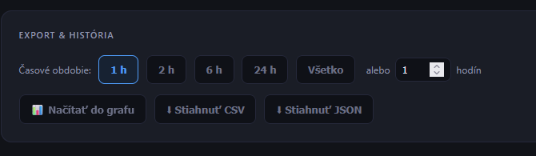
\includegraphics[width=0.85\textwidth]{images/Export_a_historia.png}
    \caption{Sekcia Export \& História – výber časového obdobia a možnosti exportu}
    \label{fig:export_historia}
\end{figure}

Backend poskytuje tri endpointy chránené prihlásením:

\begin{itemize}
    \item \texttt{GET /api/history?hours=\textit{N}} – vráti JSON pole
          posledných až 5\,000 záznamov z SQLite databázy za zvolené obdobie.
          Každý záznam obsahuje čas merania, teplotu, TEC PWM, pumpa PWM,
          aktívny mód a setpoint.
    \item \texttt{GET /api/download/csv?hours=\textit{N}} – vygeneruje a odošle
          CSV súbor s rovnakými stĺpcami vrátane strojového časového razítka
          (\texttt{created}). Názov súboru obsahuje časový rozsah
          a momentálny dátum, napr. \texttt{export\_last1h\_20250530\_143000.csv}.
    \item \texttt{GET /api/download/json?hours=\textit{N}} – rovnaký obsah
          vo formáte JSON s odsadením pre čitateľnosť.
\end{itemize}

Tlačidlom \textbf{Načítať do grafu} sa zavolá endpoint \texttt{/api/history}
a získané záznamy sa vykreslia do existujúceho grafu \emph{Priebeh merania}
na hlavnej stránke dashboardu, čo umožňuje porovnávať historické priebehy
teploty a PWM hodnôt bez nutnosti spustiť nové meranie.

\subsection{ThingsBoard integrácia}

Backend obsahuje implementovanú integráciu s cloudovou platformou \textbf{ThingsBoard}
cez MQTT protokol. Po každom prijatom meraní sú hodnoty teploty, TEC PWM, pumpa PWM,
aktívneho módu a setpointu publikované na ThingsBoard server
(\texttt{mqtt.eu.thingsboard.cloud}) pomocou access tokenu zariadenia.
Integrácia je funkčná -- dáta sú odosielané po každom prijatom meraní.

\begin{figure}[H]
  \centering
  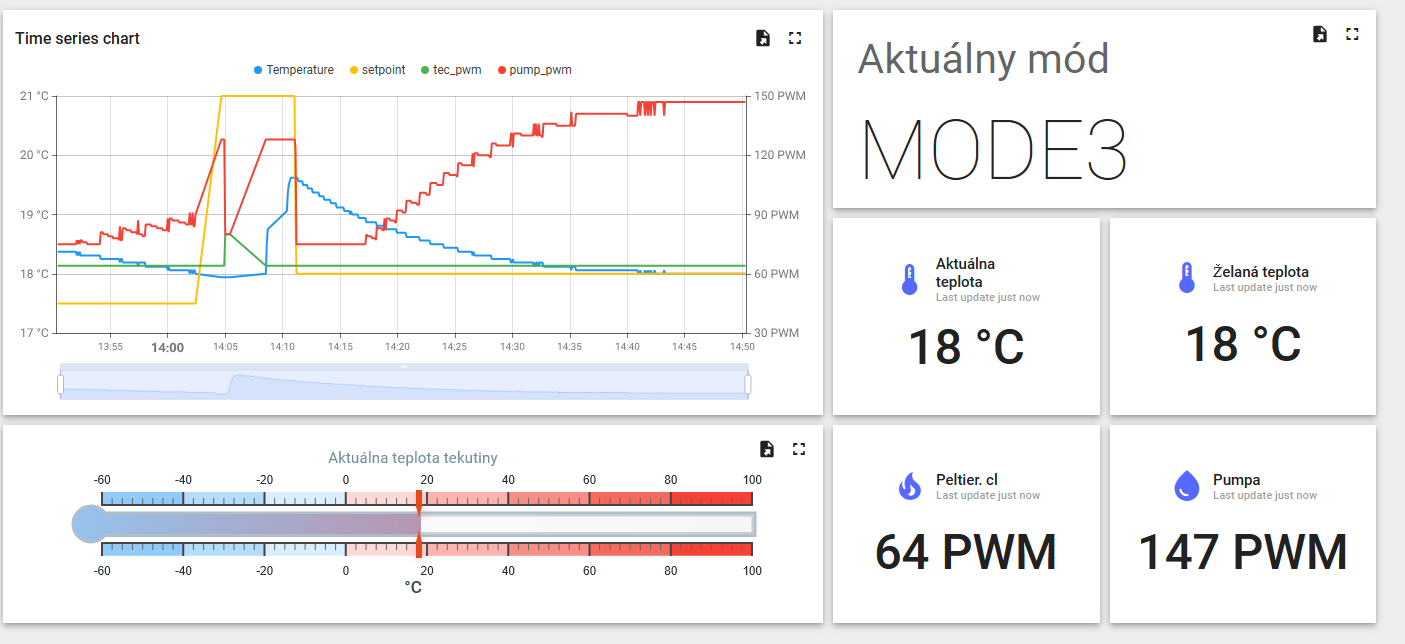
\includegraphics[width=\textwidth]{images/thingsboard.png}
  \caption{ThingsBoard dashboard -- vizualizácia telemetrie systému v cloude}
\end{figure}

\section{Frontend - Webový dashboard}

Webový dashboard je prístupný na adrese \texttt{http://147.175.105.185:5000} a tvorí
hlavné používateľské rozhranie systému. Je implementovaný v čistom HTML, CSS a
JavaScripte bez externých SPA frameworkov, pričom na vizualizáciu využíva knižnicu
\textbf{Chart.js} (grafy) a natívne \textbf{HTML5 Canvas API} (ciferníky). Komunikácia
so serverom prebieha cez WebSocket (Socket.IO klient).

\begin{figure}[H]
  \centering
  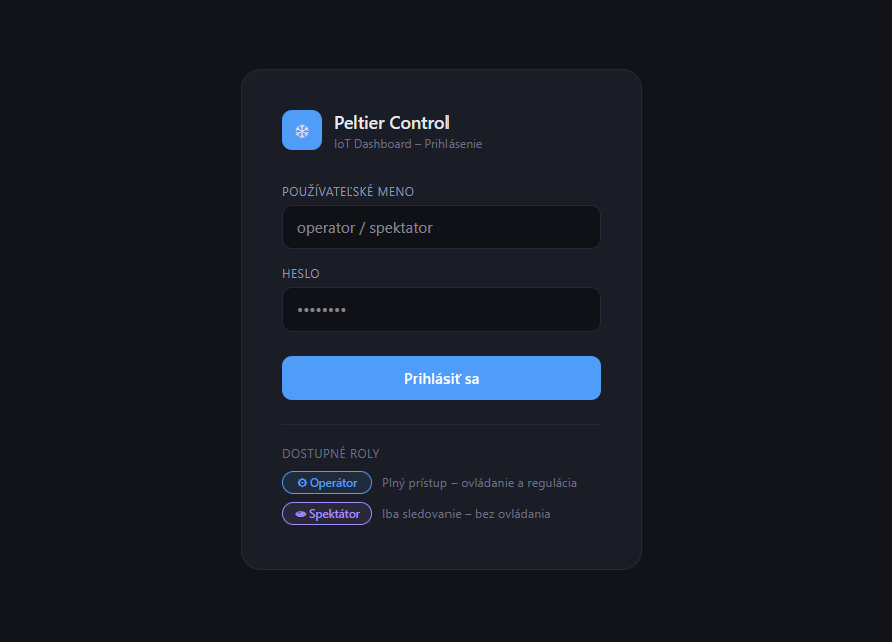
\includegraphics[width=0.6\textwidth]{images/login_screen_peltier.png}
  \caption{Prihlasovacia stránka -- Peltier Control IoT Dashboard}
\end{figure}

\subsection{Popis funkcií (Open/Start/Stop/Close)}

Ovládanie systému je rozdelené do štyroch hlavných tlačidiel umiestnených v
hornej lište dashboardu, ktoré musia byť aktivované v predpísanom poradí:

\begin{enumerate}
  \item \textbf{Open} -- inicializuje spojenie so serverom a spustí MQTT listener
        pre príjem dát z ESP32. Systém prejde do stavu \textit{inicializovaný}.
  \item \textbf{Start} -- odošle príkaz \texttt{STABILIZE} na ESP32 a spustí
        zber meraní. ESP32 nastaví TEC na 25\,\% a pumpu na 50\,\% na ustálenie
        systému.
  \item \textbf{Stop} -- zastaví meranie, odošle \texttt{STOP} na ESP32 a
        vynuluje PWM hodnoty. Systém zostane v inicializovanom stave.
  \item \textbf{Close} -- ukončí spojenie, deaktivuje systém a odošle \texttt{STOP}
        ako bezpečnostné opatrenie.
\end{enumerate}

Grafické zvýraznenie aktívneho tlačidla (napr. oranžový rámček pri \textit{Stop}
počas behu merania) poskytuje operátorovi okamžitú spätnú väzbu o stave systému.

\subsection{Grafy}

Sekcia \textbf{Priebeh merania} zobrazuje interaktívny čiarový graf vykreslený
knižnicou Chart.js. Graf zobrazuje časové priebehy:
\begin{itemize}
  \item teploty kvapaliny [°C] -- modrá krivka,
  \item setpointu [°C] -- červená prerušovaná krivka,
  \item PWM TEC alebo PWM Pumpy v závislosti od aktívneho módu -- oranžová/zelená
        krivka (pravá os Y, rozsah 0--255).
\end{itemize}

Graf si uchováva posledných 300 bodov a je aktualizovaný v reálnom čase pri
každom príchode WebSocket správy. Po načítaní stránky sa zobrazia historické dáta
z databázy (endpoint \texttt{/api/history}).

\begin{figure}[H]
  \centering
  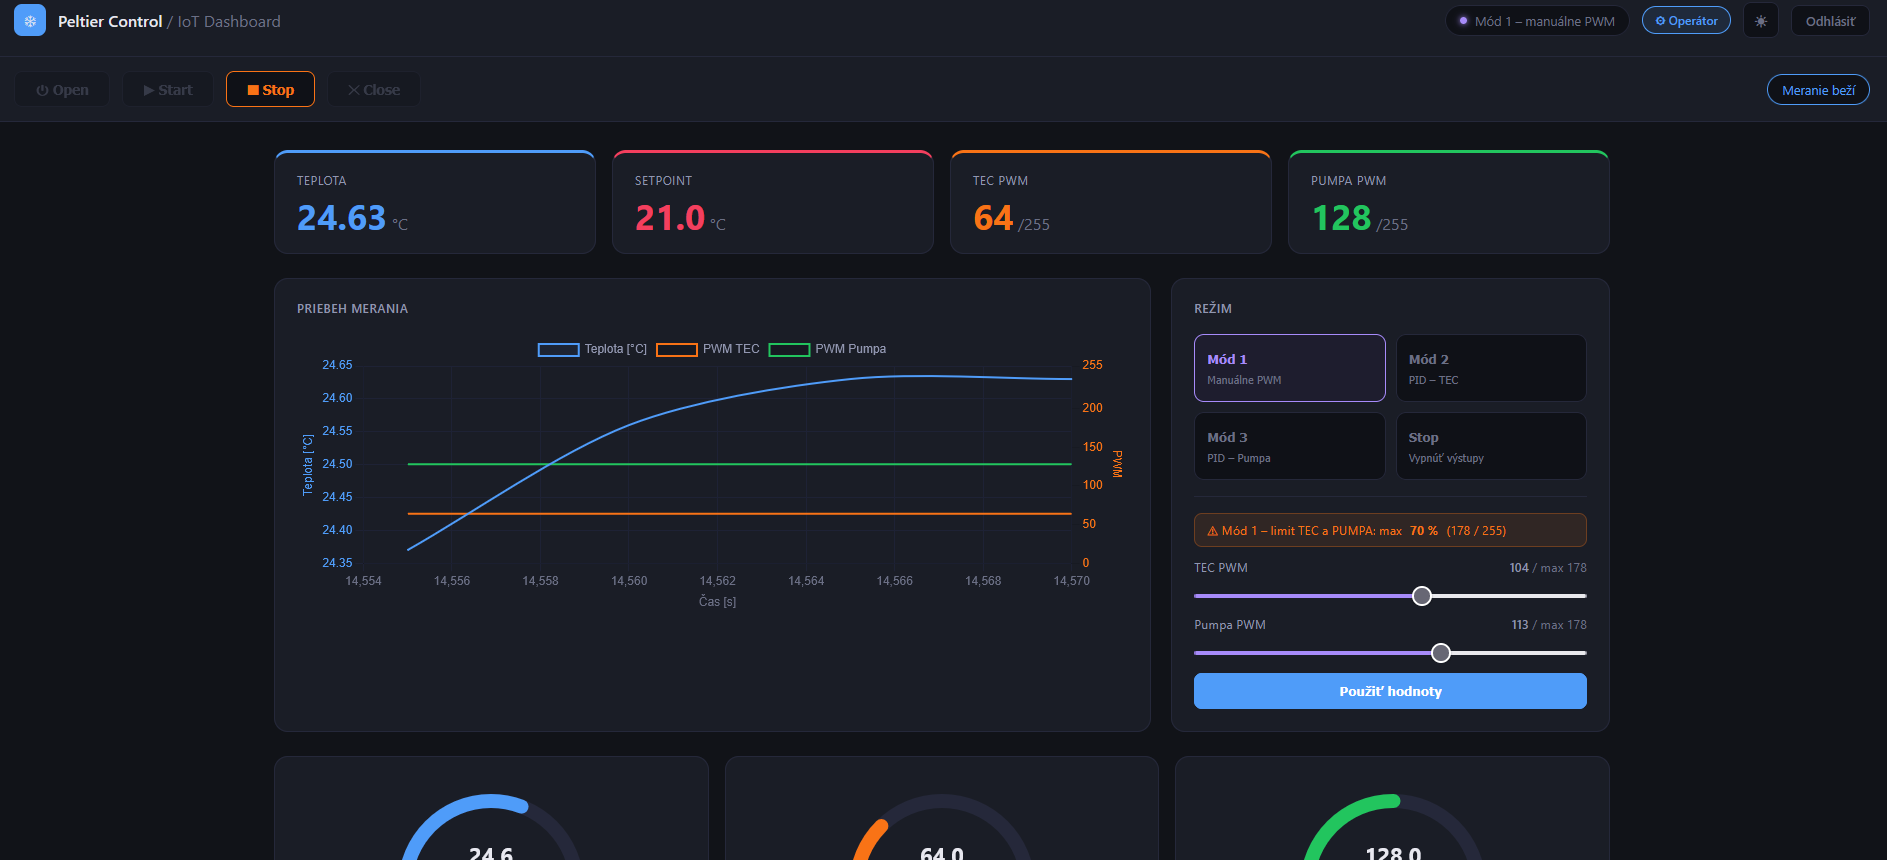
\includegraphics[width=\textwidth]{images/mod_1_peltier.png}
  \caption{Dashboard v Móde 1 (manuálne PWM) -- priebeh merania s grafom teploty a PWM}
\end{figure}

\begin{figure}[H]
  \centering
  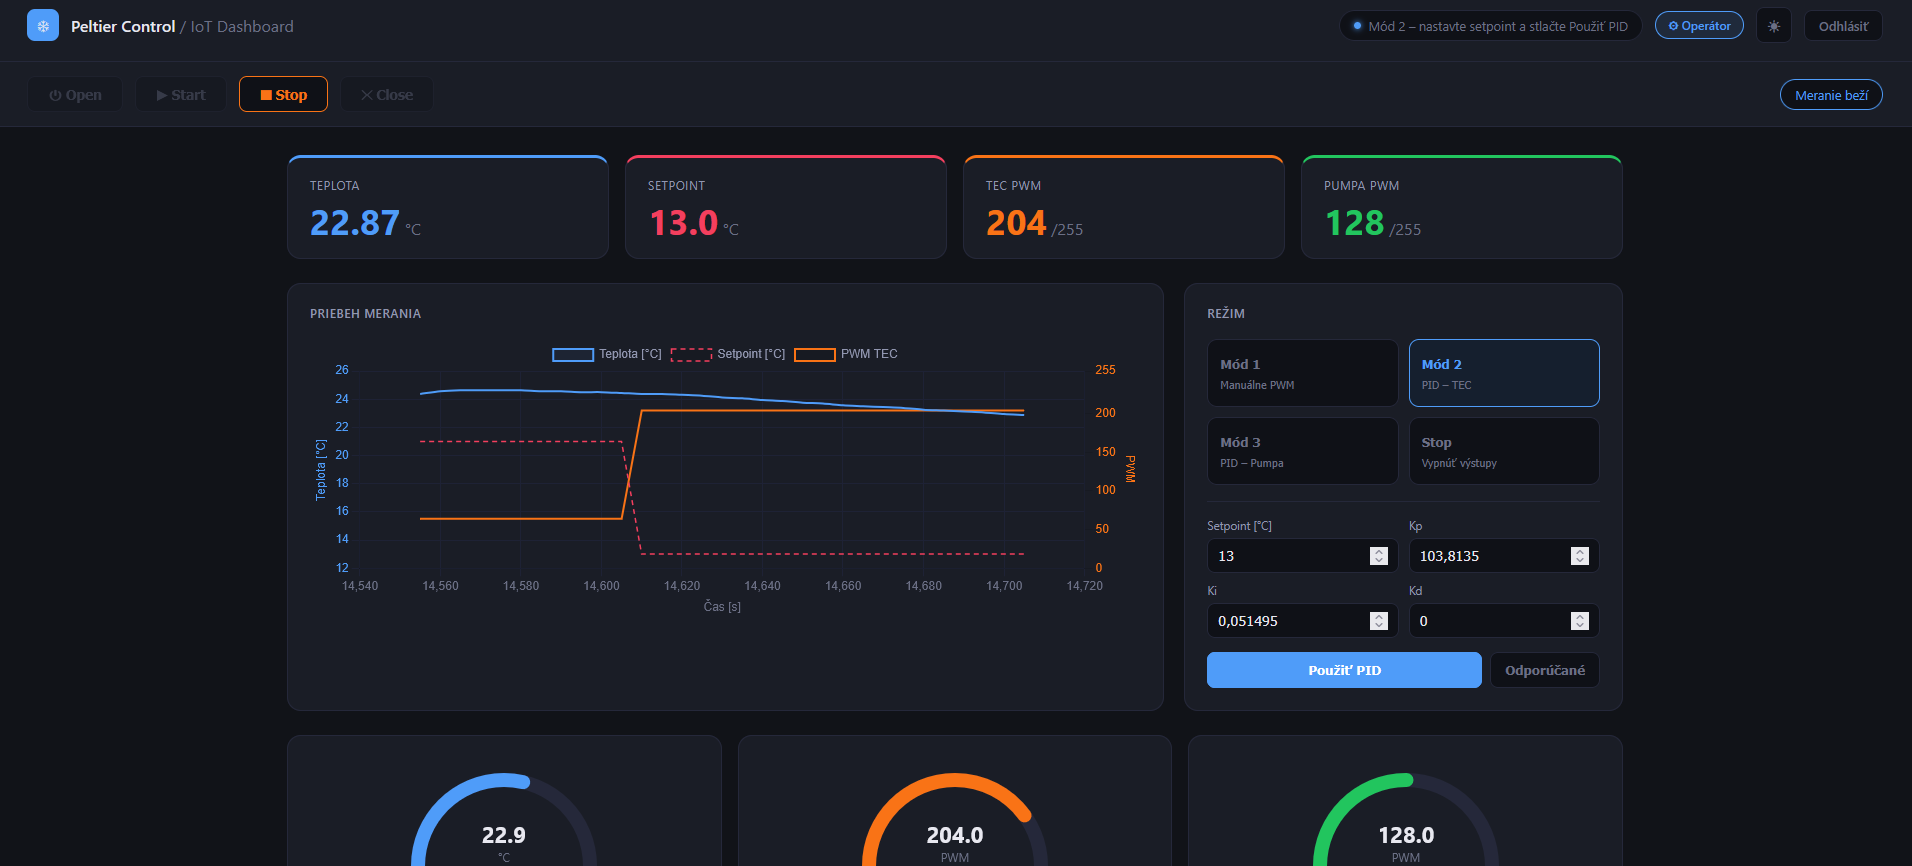
\includegraphics[width=\textwidth]{images/mod_2_peltier.png}
  \caption{Dashboard v Móde 2 (PID -- TEC) -- regulácia TEC PWM s viditeľným skokom setpointu}
\end{figure}

\begin{figure}[H]
  \centering
  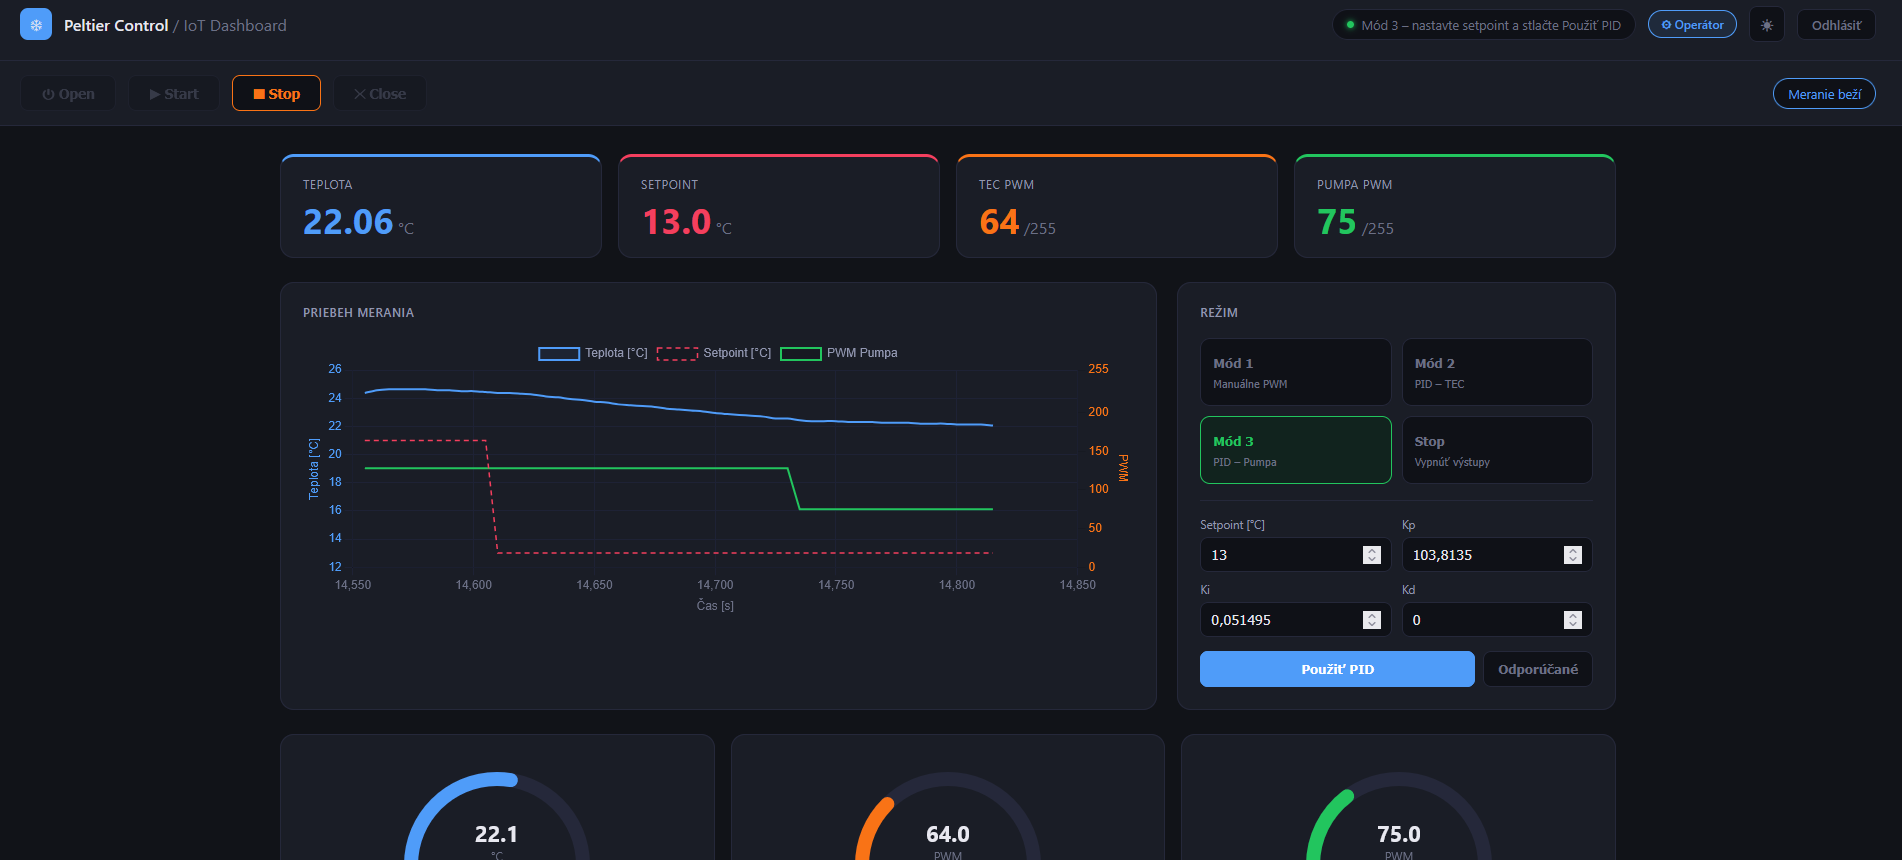
\includegraphics[width=\textwidth]{images/mod_3_peltier.png}
  \caption{Dashboard v Móde 3 (PID -- Pumpa) -- regulácia prietoku pumpy}
\end{figure}

\subsection{Ciferníky}

Pod grafom sú umiestnené tri analógové ciferníky implementované pomocou natívneho
\textbf{HTML5 Canvas API}:
\begin{itemize}
  \item \textbf{Teplota} [°C] -- modrý ciferník, rozsah 0--40\,°C,
  \item \textbf{TEC PWM} -- oranžový ciferník, rozsah 0--255,
  \item \textbf{Pumpa PWM} -- zelený ciferník, rozsah 0--255.
\end{itemize}

Ciferníky sú aktualizované synchrónne s grafom a poskytujú intuitívnu vizuálnu
reprezentáciu aktuálnych hodnôt.

\begin{figure}[H]
  \centering
  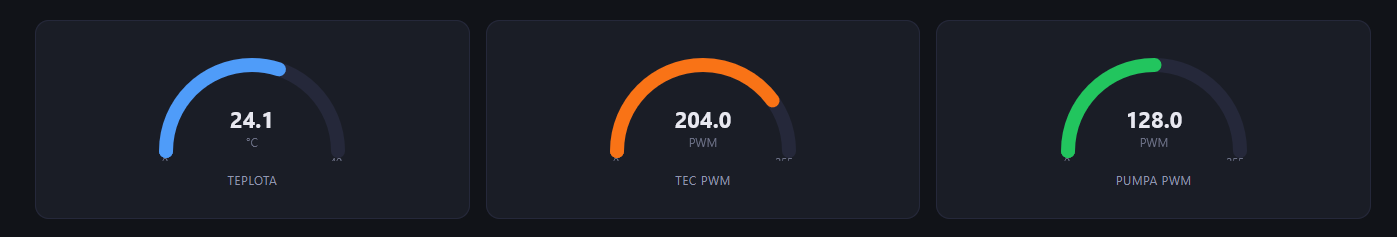
\includegraphics[width=\textwidth]{images/ciferniky_peltier.png}
  \caption{Analógové ciferníky -- teplota, TEC PWM a Pumpa PWM}
\end{figure}

\subsection{Tabuľka meraní}

Dashboard obsahuje tabuľku posledných 20 meraní. Každý riadok zobrazuje čas merania,
teplotu, TEC PWM, pumpa PWM a aktívny mód. Tabuľka je aktualizovaná v reálnom čase
pri každom príchode WebSocket správy.

\subsection{Simulácia poruchy}

Dashboard umožňuje operátorovi simulovať tepelnú poruchu pomocou tlačidla
\textbf{Simulovať poruchu}. Po stlačení sa na ESP32 odošle príkaz \texttt{HEATER\_ON},
ktorý zapne ohrievač (SSR relé) na 5 sekúnd. Po uplynutí tejto doby server automaticky
odošle \texttt{HEATER\_OFF} a ohrievač sa vypne. Počas aktívnej poruchy je tlačidlo
zablokované a zobrazuje odpočet zostávajúceho času.

\subsection{PID Panel}

Panel \textbf{Režim} na pravej strane dashboardu umožňuje operátorovi:
\begin{itemize}
  \item prepínanie medzi módmi (Mód 1, Mód 2, Mód 3, Stop),
  \item zadanie hodnôt \textit{Setpoint}, $K_p$, $K_i$, $K_d$ do číselných polí,
  \item odoslanie parametrov tlačidlom \textbf{Použiť PID},
  \item načítanie odporúčaných parametrov tlačidlom \textbf{Odporúčané}
        (rôzne hodnoty pre Mód 2 a Mód 3 podľa identifikácie systému).
\end{itemize}

Ak operátor zadá setpoint vyšší ako aktuálna teplota, server požiadavku odmietne
a odošle chybovú správu \texttt{pid\_error} -- systém totiž dokáže iba chladiť.
Aktívny mód je vizuálne zvýraznený farebným rámčekom príslušného tlačidla.

\subsection{Dashboard}

Celkový dizajn dashboardu je navrhnutý s dôrazom na prehľadnosť a použiteľnosť
v laboratórnych podmienkach. Rozhranie podporuje prepínanie medzi \textbf{tmavým
a svetlým režimom} (Dark/Light mode), pričom predvolený je tmavý. Používateľ
je informovaný o aktuálnom stave systému prostredníctvom:
\begin{itemize}
  \item farebných informačných kariet v hornej časti (Teplota, Setpoint, TEC PWM,
        Pumpa PWM) s farebnými rámčekmi podľa veličiny,
  \item stavového indikátora v pravom rohu lišty (\textit{Meranie beží} / neaktívne),
  \item zobrazeného mena a roly prihláseného používateľa,
  \item hlásenia aktívneho módu v hornej lište.
\end{itemize}

Rozhranie pre rolu \textit{spectator} je identické, no všetky ovládacie prvky
(tlačidlá, posúvače, PID polia) sú deaktivované.

\subsection{Bonusové mobilné UI}

Webový dashboard je plne responzívny a prispôsobený pre používanie na mobilných zariadeniach.
Pri šírke obrazovky do 768\,px sa aktivuje mobilné rozloženie: hlavná dvojstĺpcová plocha
sa zjednoduší na jednoduché karty a v spodnej časti obrazovky sa zobrazí fixná
navigačná lišta s ikonami.

Spodná navigácia obsahuje štyri záložky, medzi ktorými sa prepína funkciou \texttt{mobileTab()}
implementovanou priamo v JavaScripte frontendu:

\begin{itemize}
    \item \textbf{Live} – zobrazuje aktuálne hodnoty teploty, setpointu, TEC PWM a pumpy PWM
          v prehľadných kartách spolu s grafom priebehu merania (obr.~\ref{fig:mob_live}),
    \item \textbf{Ovládanie} – panel pre výber režimu (Mód 1--3, Stop) a zadanie parametrov
          setpointu a PID regulátora vrátane tlačidiel \emph{Použiť PID} a \emph{Odporúčané}
          (obr.~\ref{fig:mob_ovladanie}),
    \item \textbf{História} – tabuľka posledných meraní a sekcia Export \& História
          s výberom časového obdobia, načítaním dát do grafu a stiahnutím CSV súboru
          (obr.~\ref{fig:mob_historia}),
    \item \textbf{Meranie} – analógové ciferníky teploty, TEC PWM a pumpy PWM vykreslené
          pomocou natívneho HTML5 Canvas API.
\end{itemize}

Na mobilnom zariadení je v danom momente zobrazená vždy len aktívna záložka
(\texttt{display: block}), ostatné sú skryté (\texttt{display: none}), čím sa
eliminuje zbytočné rolovanie a zachováva sa prehľadnosť rozhrania.

\begin{figure}[H]
    \centering
    \begin{minipage}[t]{0.31\textwidth}
        \centering
        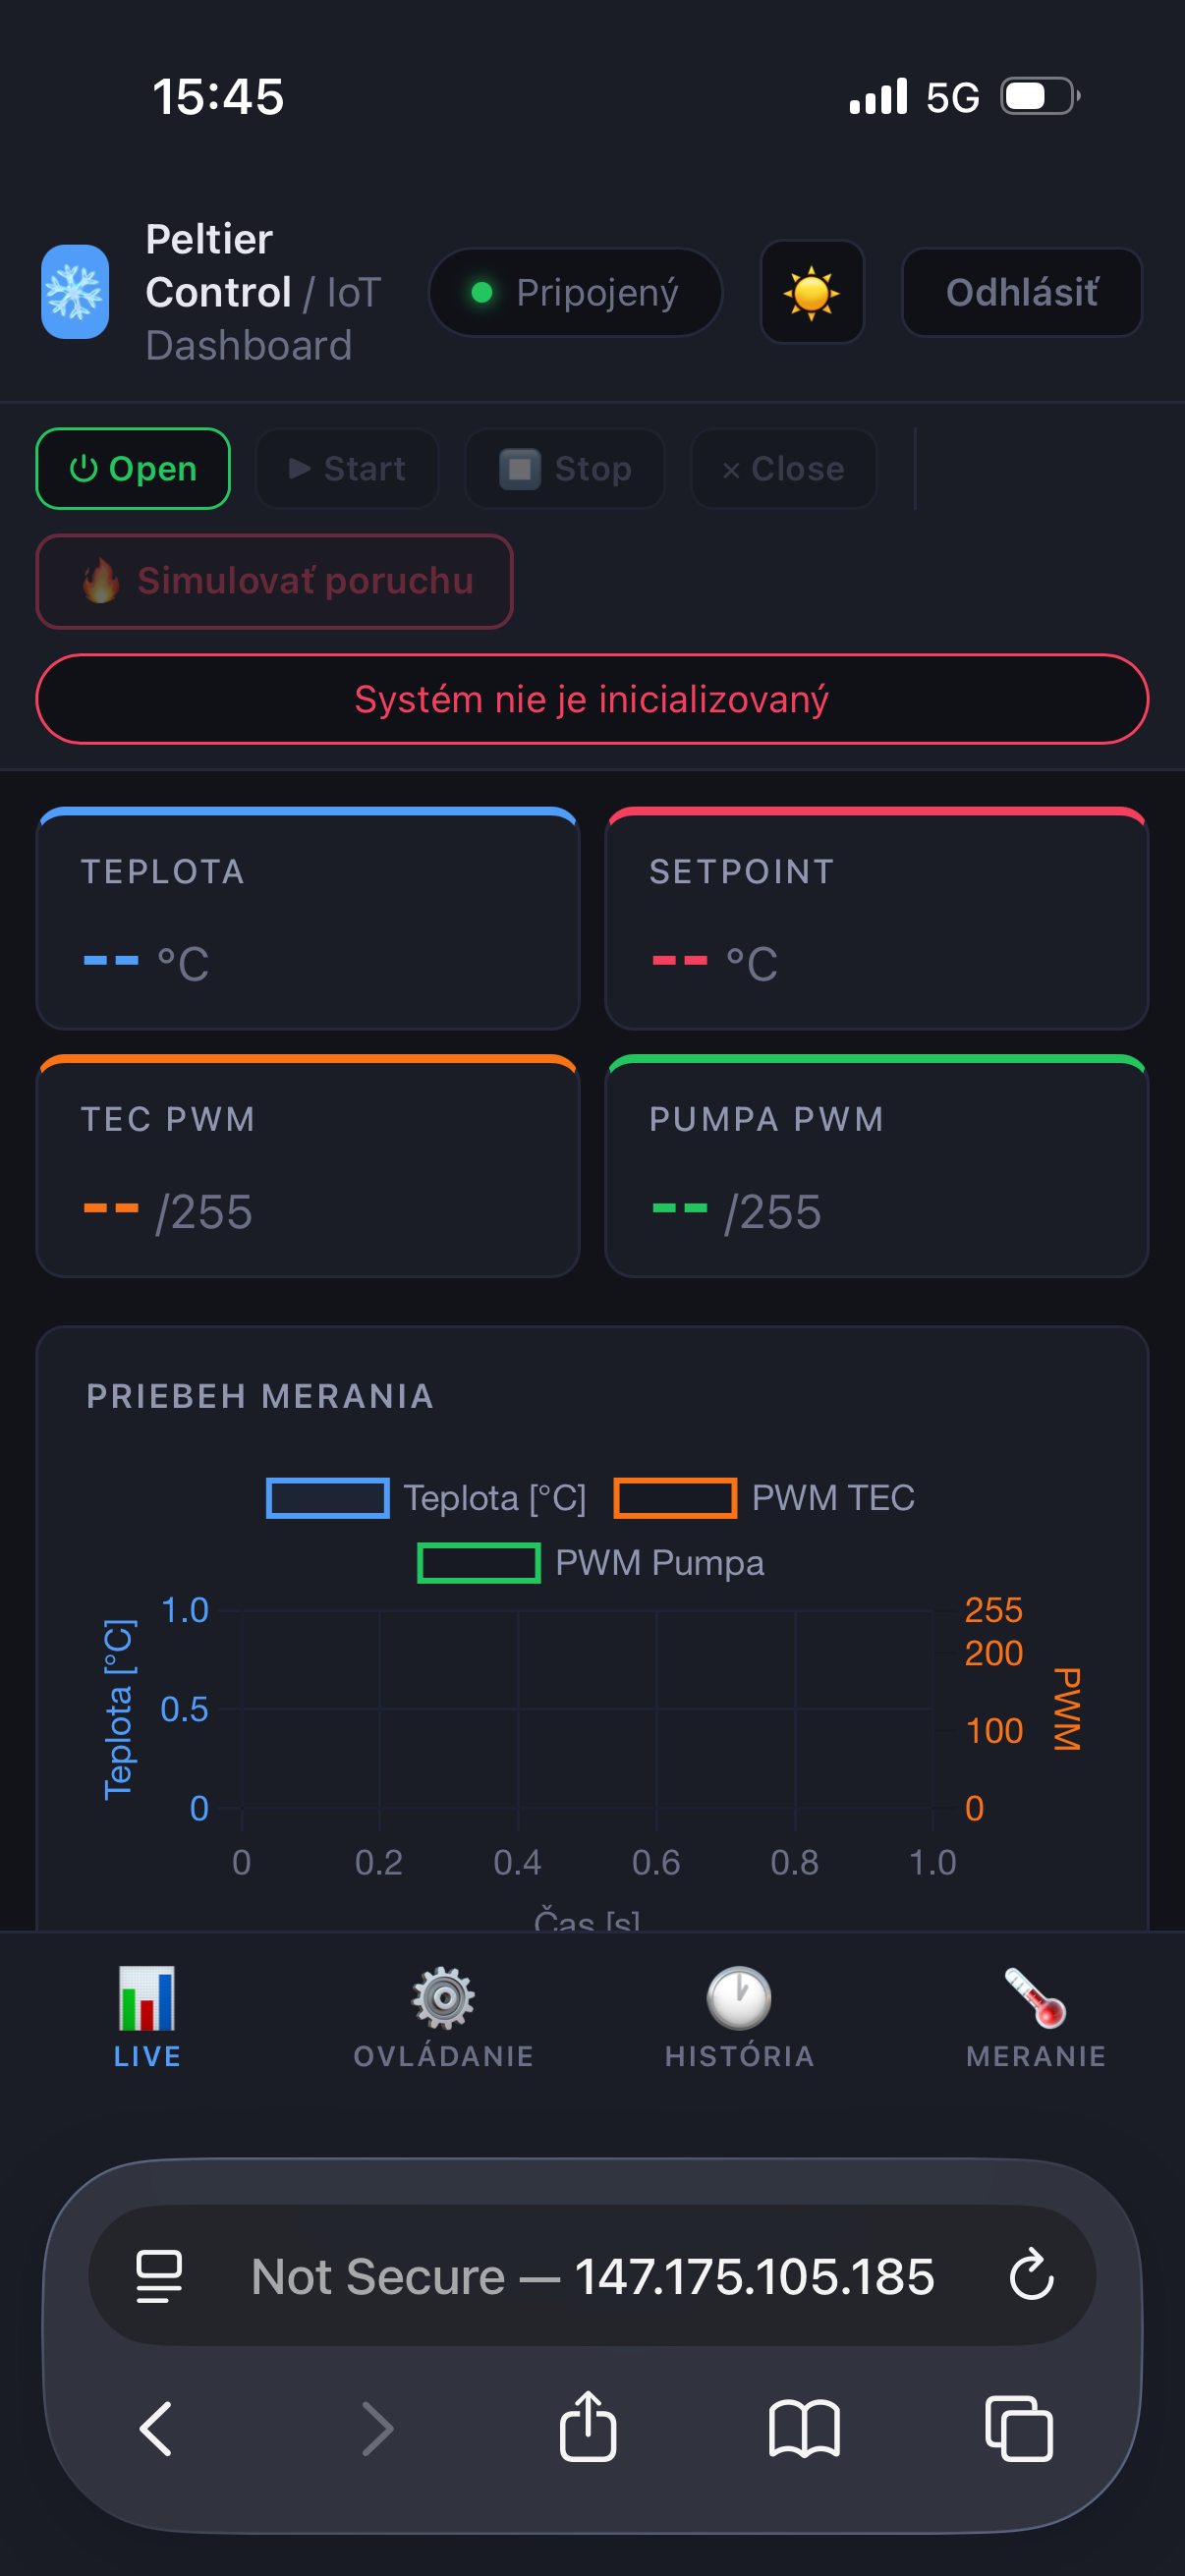
\includegraphics[width=\textwidth]{images/Mobil_UI_live.PNG}
        \caption{Mobilné UI: \\ záložka Live}
        \label{fig:mob_live}
    \end{minipage}\hfill
    \begin{minipage}[t]{0.31\textwidth}
        \centering
        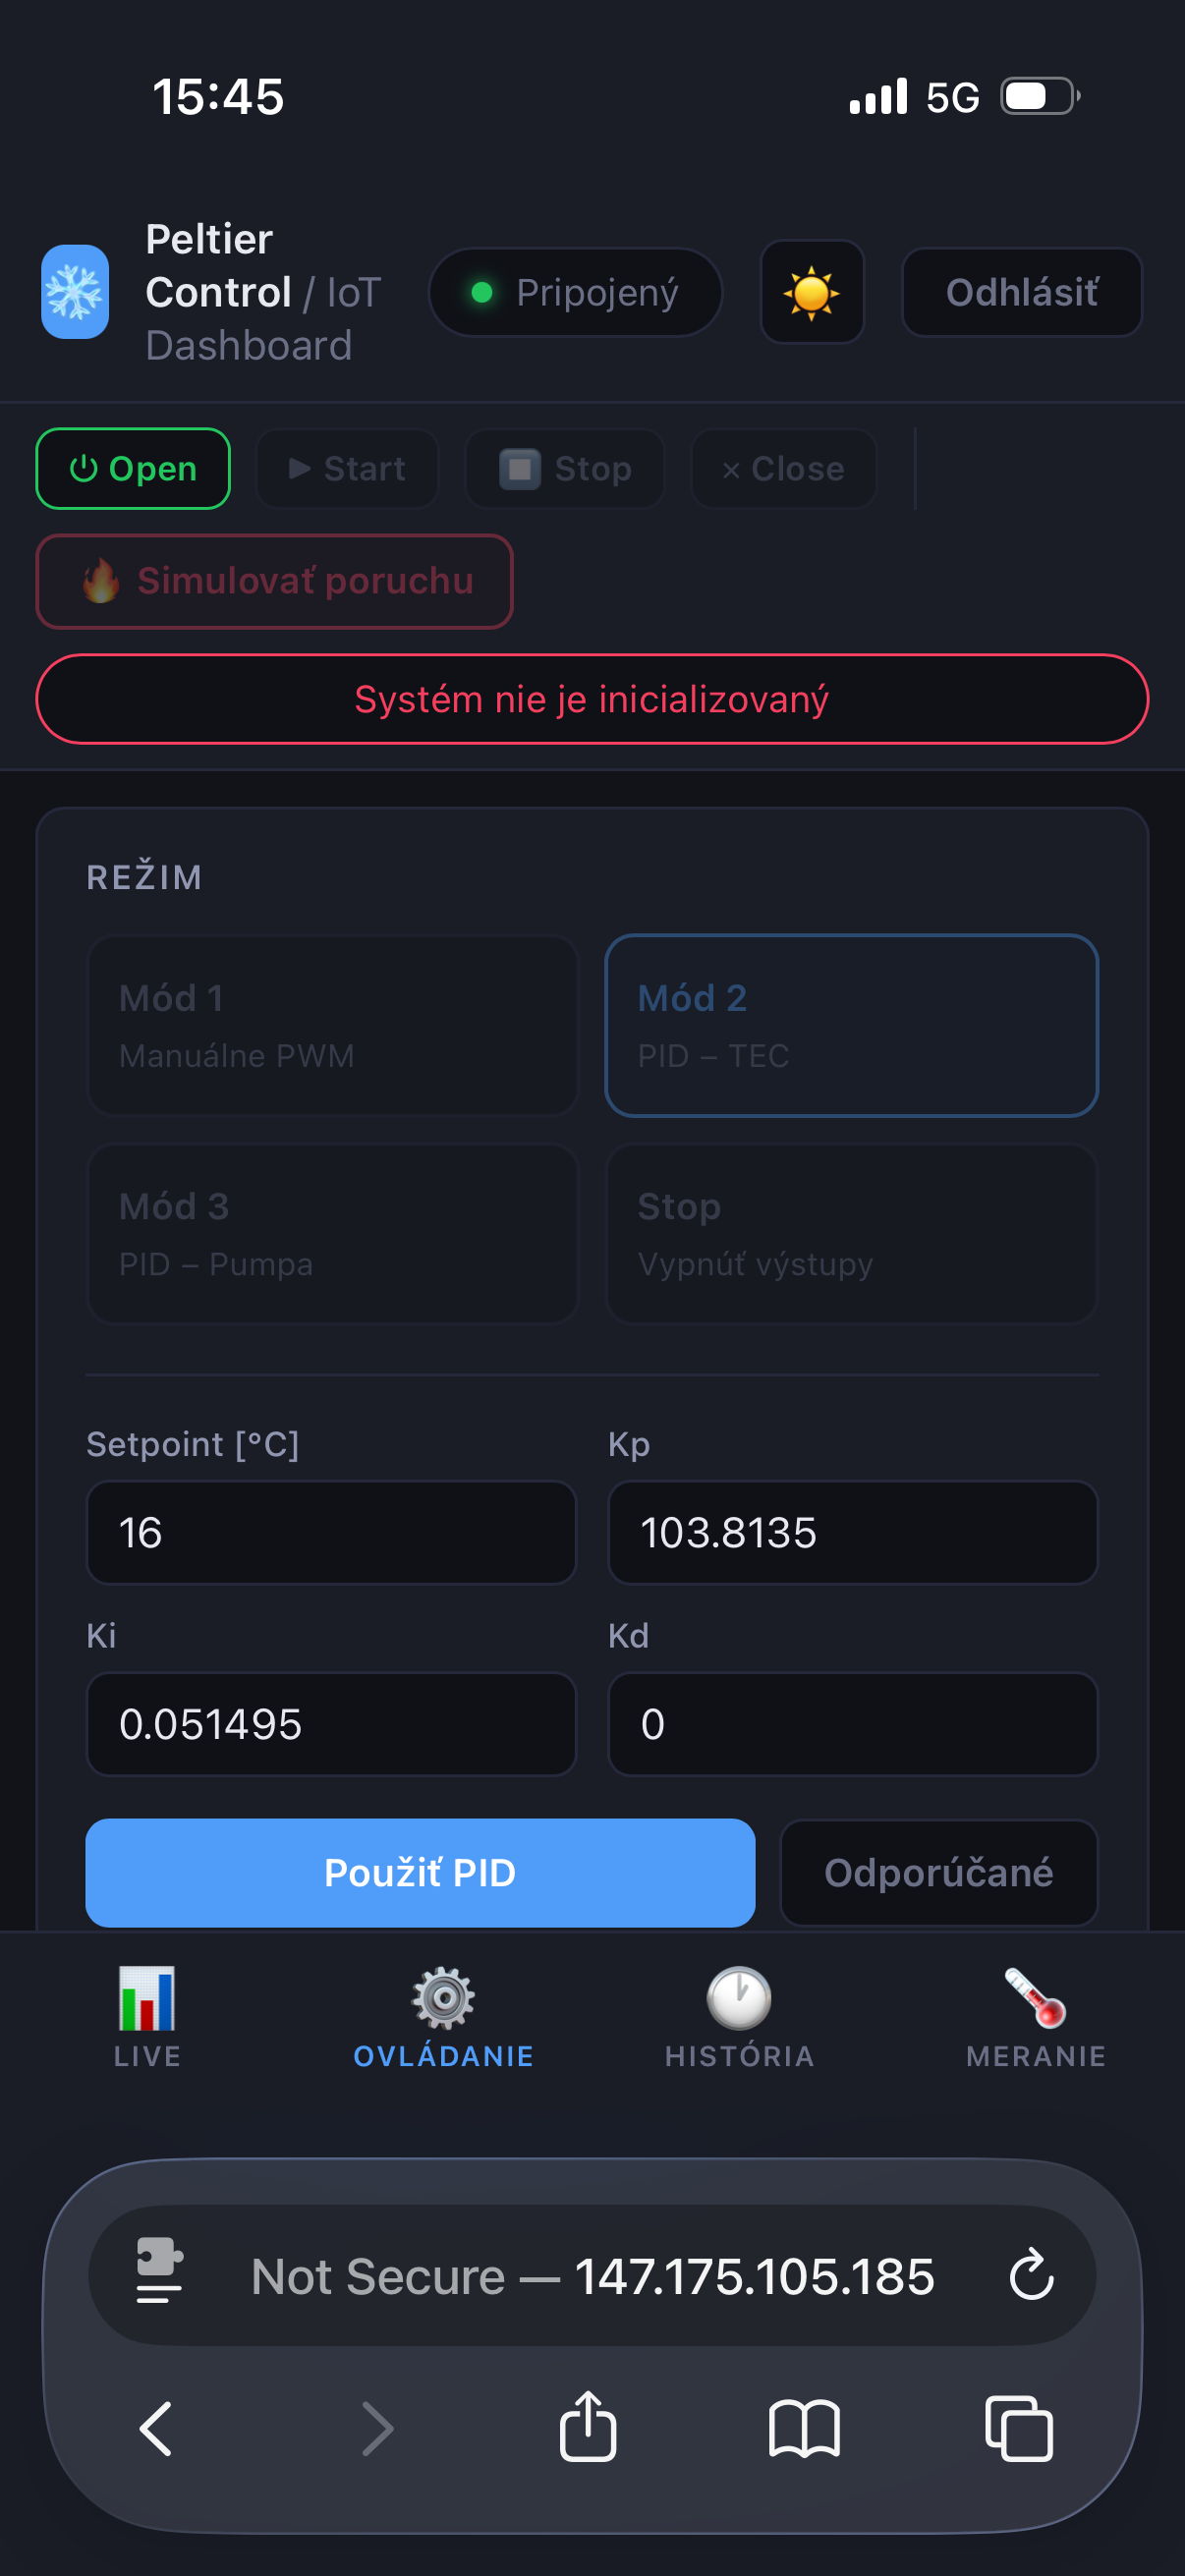
\includegraphics[width=\textwidth]{images/Mobil_UI_ovladanie.PNG}
        \caption{Mobilné UI: \\ záložka Ovládanie}
        \label{fig:mob_ovladanie}
    \end{minipage}\hfill
    \begin{minipage}[t]{0.31\textwidth}
        \centering
        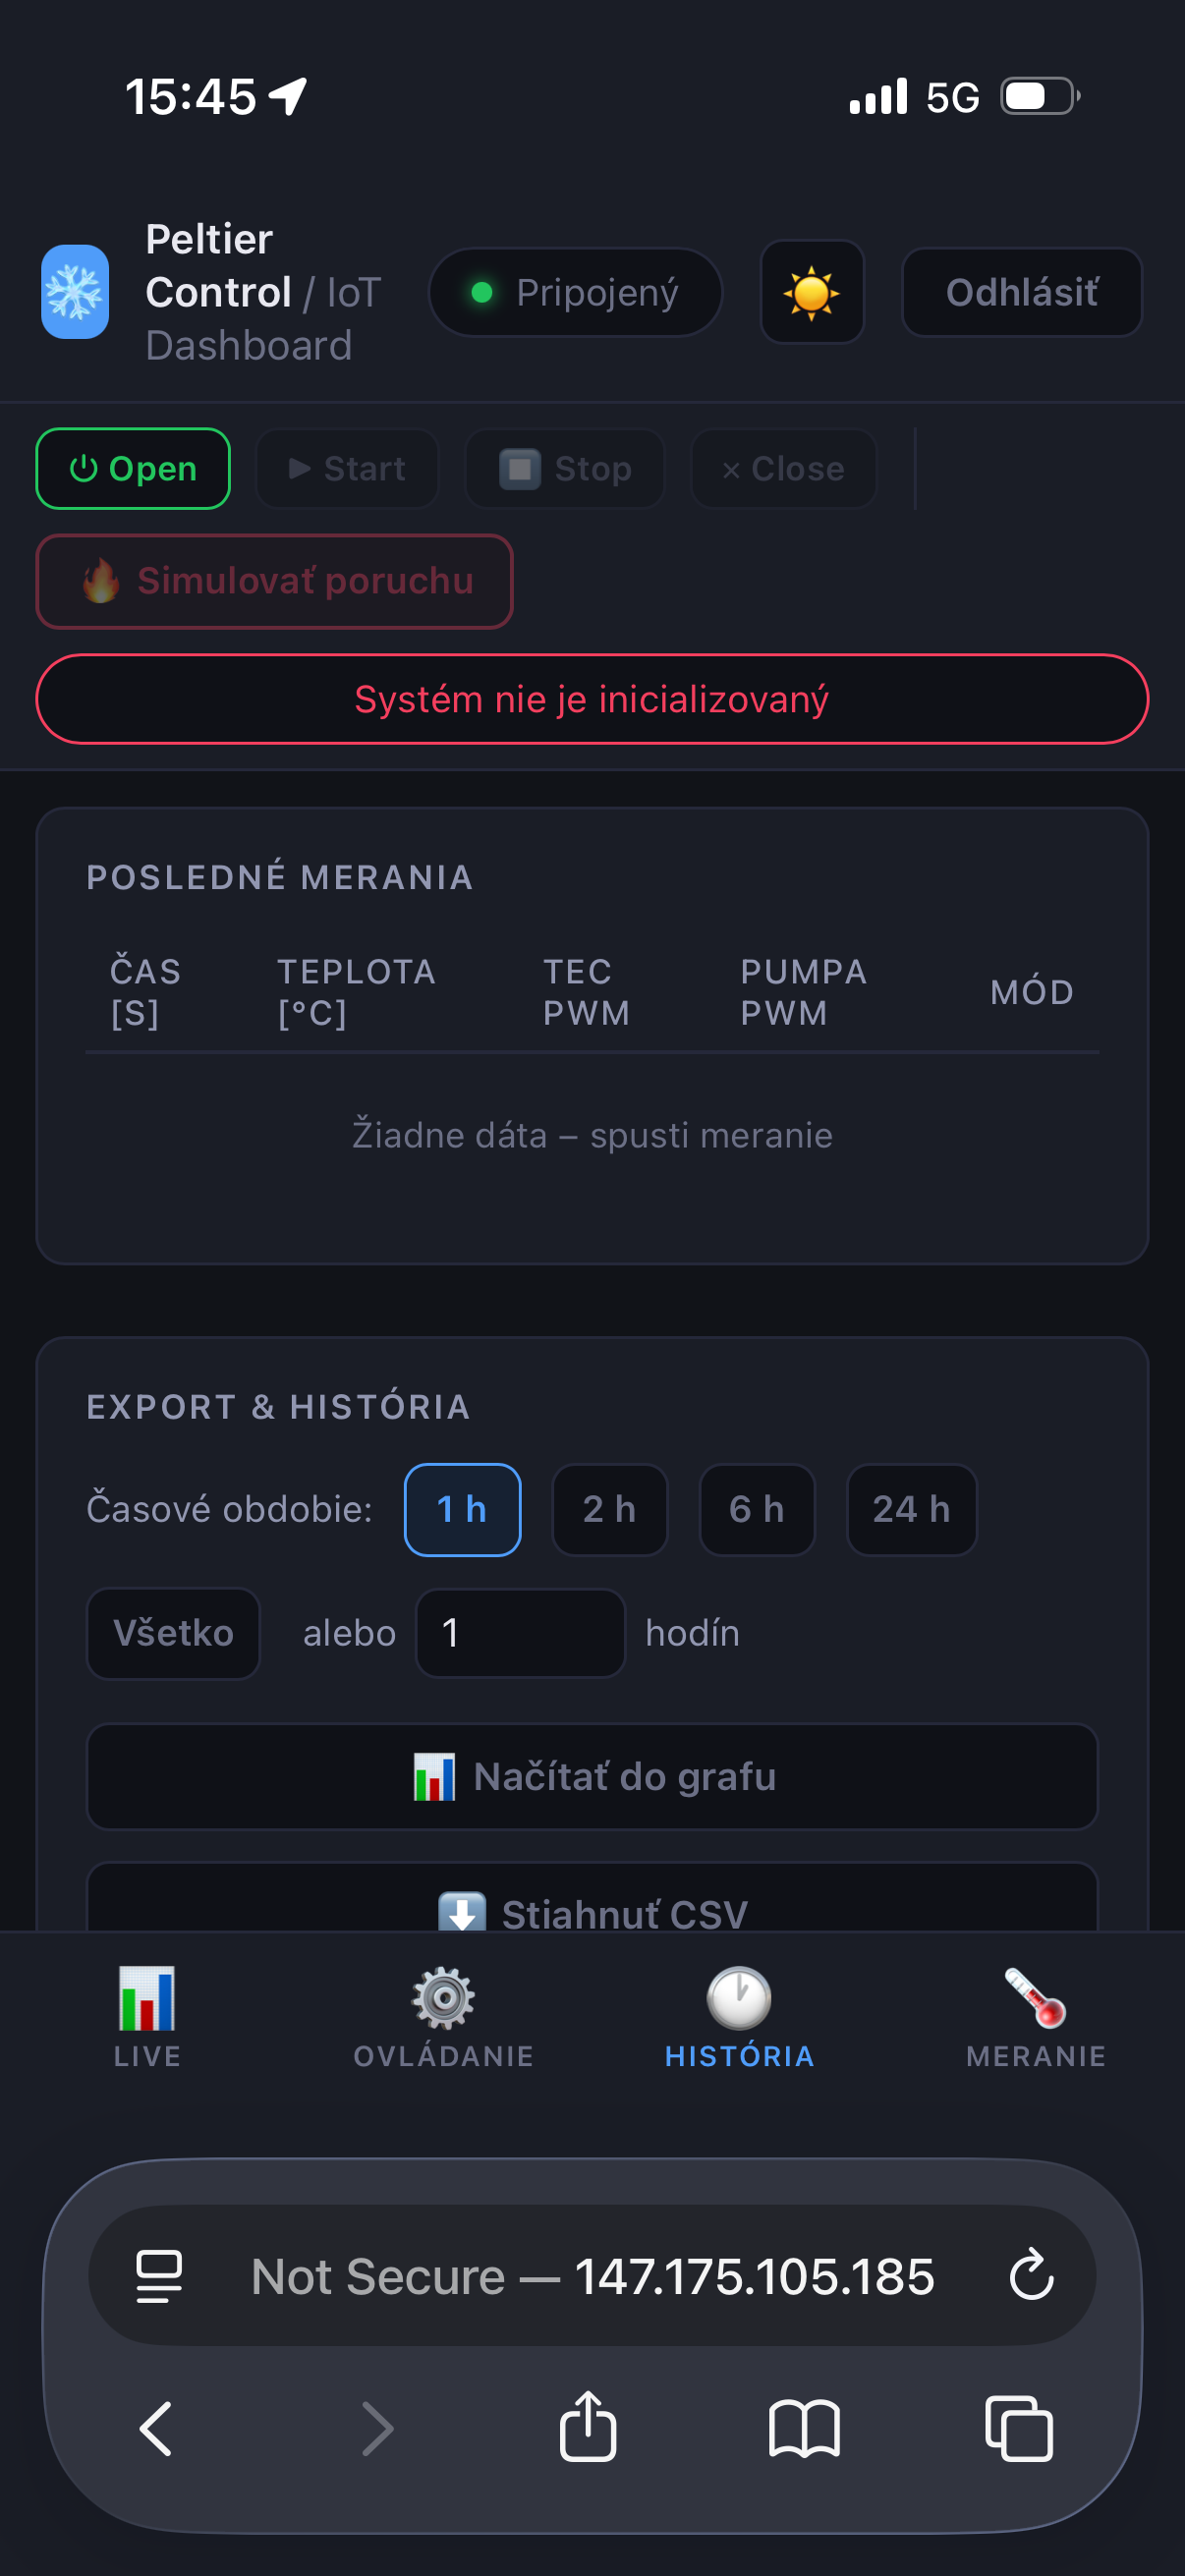
\includegraphics[width=\textwidth]{images/Mobil_UI_historia.PNG}
        \caption{Mobilné UI: \\ záložka História}
        \label{fig:mob_historia}
    \end{minipage}
\end{figure}

\section{Výsledky merania}

\subsection{Graf regulácie Mód 2}
\begin{figure}[H]
    \centering
    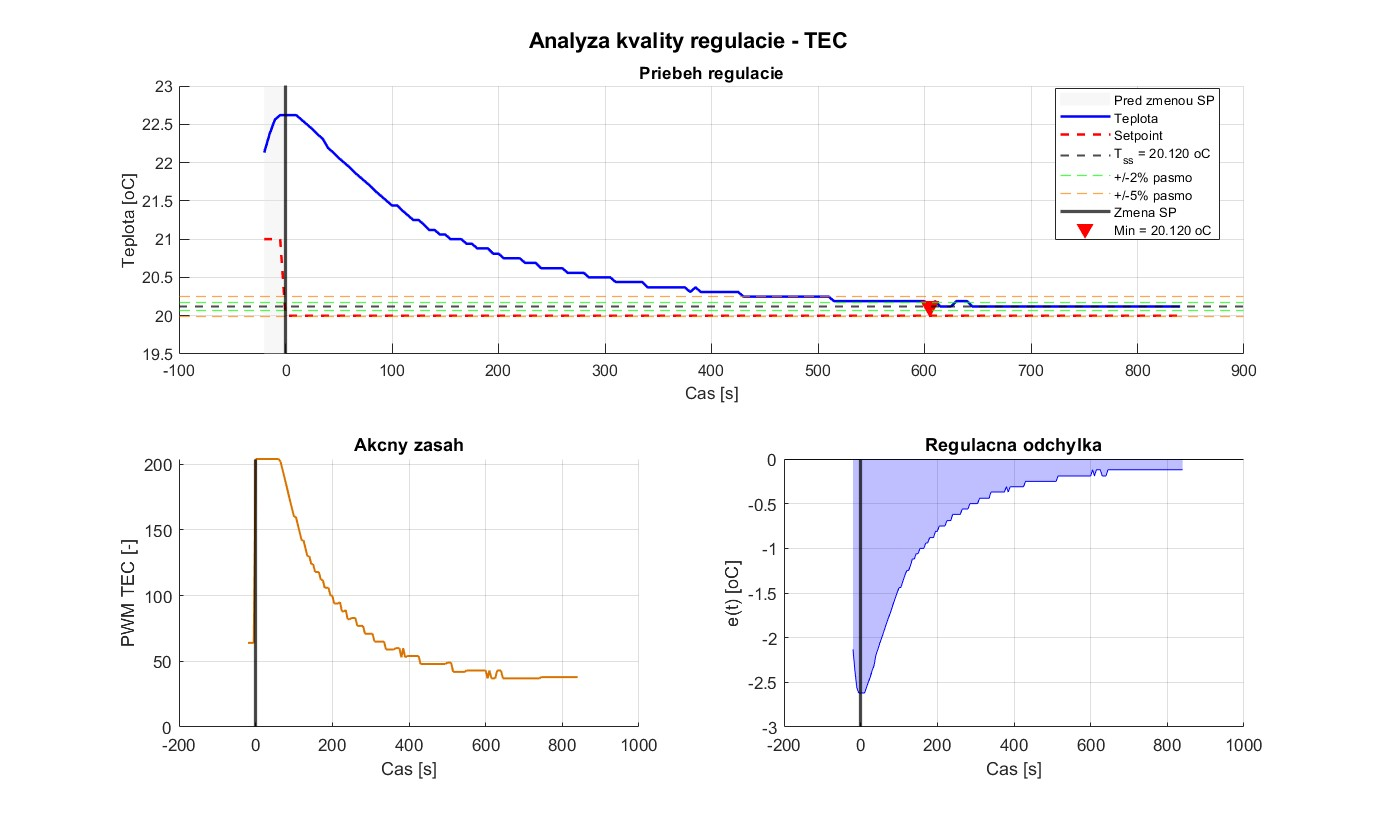
\includegraphics[width=\textwidth]{images/graf_mod2_1hod.jpg}
    \caption{Analýza kvality regulácie -- Mód 2 (meranie počas 1 hodiny)}
    \label{fig:graf_mod2}
\end{figure}

\subsection{Graf regulácie Mód 3}
\begin{figure}[H]
    \centering
    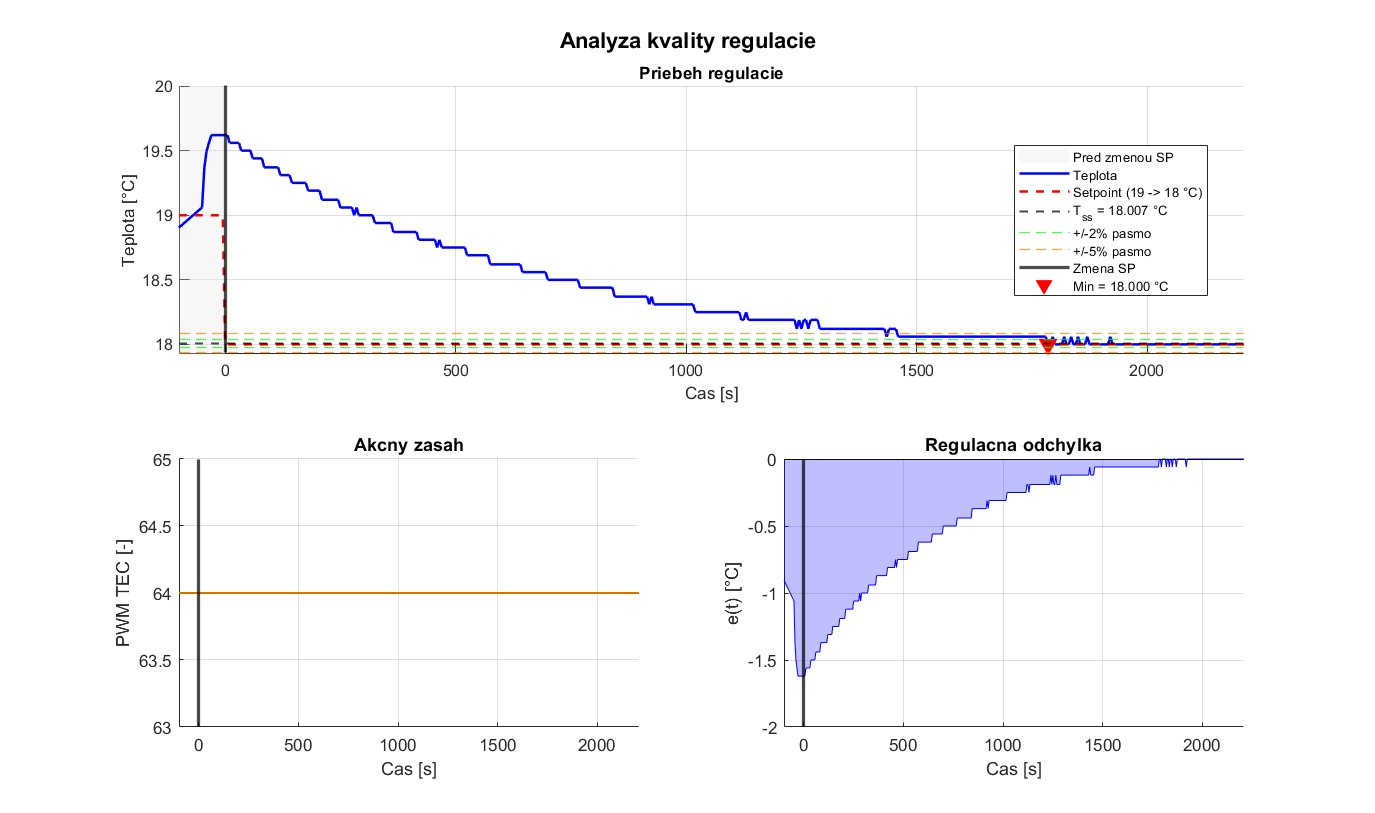
\includegraphics[width=\textwidth]{images/graf2_mod3_2hod.jpg}
    \caption{Analýza kvality regulácie -- Mód 3 (meranie počas 2 hodín)}
    \label{fig:graf_mod3}
\end{figure}

\subsection{Zhodnotenie kvality regulácie}

Meranie pre \textbf{Mód 2} bolo vykonané pri skokovej zmene setpointu z $SP_\text{old} = 21{,}0\,^\circ\text{C}$ na $SP = 20{,}0\,^\circ\text{C}$. Počiatočná teplota v momente zmeny setpointu bola $T_0 = 22{,}62\,^\circ\text{C}$. Systém sa ustálil na hodnote $T_{ss} = 20{,}12\,^\circ\text{C}$, čo predstavuje trvalú regulačnú odchýlku:
\begin{equation}
    e_{ss2} = SP - T_{ss} = 20{,}0 - 20{,}12 = -0{,}12\,^\circ\text{C}
\end{equation}
Nenulová trvalá odchýlka pri Móde 2 naznačuje, že regulátor neobsahuje integračnú zložku. Preregulovanie dosiahlo hodnotu $0\,\%$, čo znamená, že teplota neprekročila cieľový setpoint. Systém vykazuje pomalý, ale monotónny pokles teploty bez kmitania. Doba ustalenia v tolerančnom pásme $\pm 2\,\%$ bola $645\,\text{s}$.

Meranie pre \textbf{Mód 3} prebiehalo pri skokovej zmene setpointu z $SP_\text{old} = 19{,}0\,^\circ\text{C}$ na $SP = 18{,}0\,^\circ\text{C}$ s počiatočnou teplotou $T_0 = 19{,}62\,^\circ\text{C}$. Systém sa ustálil na hodnote $T_{ss} = 18{,}0067\,^\circ\text{C}$. Trvalá regulačná odchýlka tohto módu je:
\begin{equation}
    e_{ss3} = SP - T_{ss} = 18{,}0 - 18{,}0067 = -0{,}0067\,^\circ\text{C}
\end{equation}
Pri chladení v Móde 3 bolo zaznamenané minimálne preregulovanie (prekmit) na úrovni $0{,}41\,\%$, kedy teplota klesla na minimálnu hodnotu $18{,}000\,^\circ\text{C}$, čo predstavuje zanedbateľný zákmit. Prvé dosiahnutie setpointu nastalo v čase $1785{,}0\,\text{s}$.

Namerané parametre prechodového deja pre oba módy sú zhrnuté v tabuľke~\ref{tab:kvalita}.

\begin{table}[H]
\centering
\caption{Parametre kvality regulácie -- porovnanie Mód 2 a Mód 3}
\label{tab:kvalita}
\begin{tabular}{lccc}
\hline
\textbf{Parameter} & \textbf{Jednotka} & \textbf{Mód 2} & \textbf{Mód 3} \\
\hline
Setpoint skok ($SP_\text{old} \rightarrow SP$) & $^\circ\text{C}$ & $21{,}0 \rightarrow 20{,}0$ & $19{,}0 \rightarrow 18{,}0$ \\
Počiatočná teplota $T_0$    & $^\circ\text{C}$   & $22{,}62$    & $19{,}62$    \\
Ustálená hodnota $T_{ss}$   & $^\circ\text{C}$   & $20{,}12$    & $18{,}0067$  \\
Trvalá odchýlka $e_{ss}$    & $^\circ\text{C}$   & $-0{,}12$    & $-0{,}0067$  \\
Preregulovanie              & \%                 & $0{,}00$     & $0{,}41$     \\
Čas prvého dosiahnutia SP   & s                  & --           & $1785{,}0$   \\
Čas nábehu (10\,\%--90\,\%) & s                  & $310{,}0$    & $1180{,}0$   \\
Doba ustalenia ($\pm$2\,\%) & s                  & $645{,}0$    & $1925{,}0$   \\
Doba ustalenia ($\pm$5\,\%) & s                  & $515{,}0$    & $1460{,}0$   \\
IAE                         & $^\circ\text{C}\cdot\text{s}$       & $501{,}45$       & $911{,}35$       \\
ISE                         & $^\circ\text{C}^2\cdot\text{s}$     & $654{,}68$       & $806{,}62$       \\
ITAE                        & $^\circ\text{C}\cdot\text{s}^2$     & $98\,692{,}00$   & $429\,640{,}50$  \\
\hline
\end{tabular}
\end{table}

\subsection{Porovnanie módov}

Z porovnania výsledkov v tabuľke~\ref{tab:kvalita} vyplýva, že oba regulačné módy vykazujú zásadne odlišné dynamické vlastnosti.

\textbf{Mód 2} je z hľadiska rýchlosti prechodového deja podstatne agresívnejší. Čas nábehu ($310\,\text{s}$) aj doba ustalenia pre $\pm2\,\%$ pásmo ($645\,\text{s}$) sú výrazne kratšie ako pri Móde 3. Daňou za túto rýchlosť je však značná trvalá regulačná odchýlka ($e_{ss} = -0{,}12\,^\circ\text{C}$), čo svedčí o nedostatočnom zosilnení alebo chýbajúcej integračnej zložke schopnej eliminovať tento offset pri danej záťaži.

Naopak, \textbf{Mód 3} uprednostňuje presnosť pred rýchlosťou. Dokáže eliminovať trvalú regulačnú odchýlku na takmer nulovú hodnotu ($-0{,}0067\,^\circ\text{C}$), čo je z pohľadu presnosti vynikajúci výsledok. Systém sa však k novému setpointu približuje omnoho pomalšie, čo potvrdzuje čas nábehu ($1180\,\text{s}$) a doba ustalenia ($1925\,\text{s}$). Pomalý nábeh a dlhé pretrvávanie regulačnej odchýlky sa negatívne prejavilo na integrálnych kritériách. Kritériá IAE ($911{,}35$) a najmä ITAE ($429\,640{,}50$), ktoré výrazne penalizujú odchýlku pretrvávajúcu v dlhom čase, sú pri Móde 3 podstatne vyššie ako pri Móde 2. Akčný zásah (PWM TEC) bol počas celej doby udržiavaný na konštantnej hodnote, čo zodpovedá ustálenému príkonu chladiaceho prvku v danej pracovnej oblasti.

\section{Používateľská príručka}

\subsection{Spustenie systému (krok za krokom)}

\begin{enumerate}
    \item Pripojiť sa na Raspberry Pi cez SSH: \texttt{ssh misa26@147.175.105.185}
    \item Spustiť Flask server: \texttt{cd ~/peltier \&\& python3 app.py}
    \item Otvoriť dashboard v prehliadači: \texttt{http://147.175.105.185:5000}
    \item Prihlásiť sa ako \textit{operator} (plný prístup) alebo \textit{spectator} (sledovanie)
    \item Stlačiť \textbf{Open} → \textbf{Start} → vybrať mód regulácie
\end{enumerate}

\subsection{Popis tlačidiel dashboardu}

\begin{table}[H]
\centering
\renewcommand{\arraystretch}{1.3}
\begin{tabular}{|l|l|}
\hline
\textbf{Tlačidlo} & \textbf{Funkcia} \\
\hline
Open     & Inicializácia spojenia s ESP32 \\
Start    & Spustenie merania (ESP32 prechádza do stabilizácie) \\
Stop     & Zastavenie merania, vypnutie výstupov \\
Close    & Ukončenie spojenia, bezpečnostný STOP \\
Mód 1    & Manuálne nastavenie PWM cez posúvače \\
Mód 2    & PID regulácia cez Peltierov článok \\
Mód 3    & PID regulácia cez pumpu \\
Simulovať poruchu & Zapnutie ohrievača na 5 sekúnd \\
\hline
\end{tabular}
\caption{Prehľad tlačidiel dashboardu}
\end{table}

\subsection{Nastavenie PID parametrov}

V paneli \textbf{Režim} zadajte hodnoty \textit{Setpoint}, $K_p$, $K_i$, $K_d$ a potvrďte tlačidlom \textbf{Použiť PID}. Tlačidlo \textbf{Odporúčané} načíta prednastavené parametre podľa aktívneho módu. Setpoint nesmie byť vyšší ako aktuálna teplota -- systém dokáže iba chladiť.

\subsection{Export dát}

V sekcii \textbf{Export \& História} zvolte časové obdobie (1\,h, 2\,h, 6\,h, 24\,h alebo vlastný počet hodín) a stiahnite dáta tlačidlom \textbf{Stiahnuť CSV} alebo \textbf{Stiahnuť JSON}. Tlačidlo \textbf{Načítať do grafu} zobrazí históriu priamo v grafe dashboardu.

\section{Vývojárska príručka}

\subsection{Štruktúra repozitára}

Zdrojový kód je dostupný na \url{https://github.com/StinkyMyers/iot-peltier-temperature-control}.

\begin{table}[H]
\centering
\renewcommand{\arraystretch}{1.3}
\begin{tabular}{|l|l|}
\hline
\textbf{Priečinok} & \textbf{Obsah} \\
\hline
\texttt{esp32/} & Firmvér ESP32 (PlatformIO projekt) \\
\texttt{flask/} & Flask backend, šablóny, databáza \\
\texttt{ident/} & Identifikačné skripty a namerané dáta \\
\texttt{hw/}    & Schéma zapojenia \\
\texttt{docs/}  & LaTeX dokumentácia \\
\hline
\end{tabular}
\caption{Štruktúra repozitára}
\end{table}

\subsection{Inštalácia závislostí}

Na Raspberry Pi:
\begin{verbatim}
pip3 install flask flask-socketio flask-sqlalchemy
        paho-mqtt --break-system-packages
sudo apt install mosquitto mosquitto-clients -y
\end{verbatim}

Pre ESP32 sú závislosti definované v \texttt{platformio.ini}:
\texttt{OneWire}, \texttt{DallasTemperature}, \texttt{PubSubClient}.

\subsection{Konfigurácia (WiFi, MQTT, port)}

V súbore \texttt{esp32/src/main.cpp} nastavte:
\begin{verbatim}
const char* WIFI_SSID   = "nazov_siete";
const char* WIFI_PASS   = "heslo";
const char* MQTT_SERVER = "147.175.105.185";
\end{verbatim}

\subsection{Spustenie backendu}

Backend je nakonfigurovaný ako systemd služba, ktorá sa automaticky spustí po štarte Raspberry Pi.

\begin{verbatim}
# Spustenie
sudo systemctl start mosquitto
sudo systemctl start peltier

# Zastavenie
sudo systemctl stop peltier

# Stav
sudo systemctl status peltier
\end{verbatim}

Dashboard je následne dostupný na \texttt{http://147.175.105.185:5000}.

\section{Záver}

Cieľom projektu bolo navrhnúť a realizovať kompletný IoT systém na reguláciu teploty chladiacej kvapaliny pomocou Peltierovho článku. Všetky stanovené ciele boli úspešne splnené.

Boli identifikované dva regulačné módy systému. Pre Mód~2 (regulácia TEC) bola použitá jednobodová metóda identifikácie a parametre PID regulátora boli stanovené heuristicky v prostredí Simulink. Pre Mód~3 (regulácia pumpy) bola použitá dvojbodová metóda a parametre PI regulátora boli vypočítané analyticky metódou SIMC.

Merania preukázali, že \textbf{Mód 2} dosahuje rýchlejší prechodový dej (doba ustalenia $645\,\text{s}$) za cenu trvalej regulačnej odchýlky $-0{,}12\,^\circ\text{C}$. \textbf{Mód 3} dosahuje výrazne vyššiu presnosť (odchýlka $-0{,}0067\,^\circ\text{C}$) pri pomalšom nábehu (doba ustalenia $1925\,\text{s}$).

Implementovaný IoT backend na Raspberry Pi zabezpečuje príjem dát z ESP32 cez MQTT, archiváciu do SQLite databázy, real-time distribúciu cez WebSocket a cloudovú vizualizáciu cez ThingsBoard. Webový dashboard poskytuje plnohodnotné rozhranie pre vzdialené ovládanie a monitoring systému s autentifikáciou a rozlíšením rolí operátor/spektátor.

\begin{thebibliography}{9}

\bibitem{tec}
TEC1-12706 Datasheet.
\textit{Thermoelectric Cooler Module}.
Dostupné na: \url{https://www.tec-thermoelectric.com}

\bibitem{ds18b20}
Maxim Integrated.
\textit{DS18B20 Programmable Resolution 1-Wire Digital Thermometer}.
Dostupné na: \url{https://www.analog.com/media/en/technical-documentation/data-sheets/ds18b20.pdf}

\bibitem{flask}
Pallets Projects.
\textit{Flask Documentation}.
Dostupné na: \url{https://flask.palletsprojects.com}

\bibitem{socketio}
Miguel Grinberg.
\textit{Flask-SocketIO Documentation}.
Dostupné na: \url{https://flask-socketio.readthedocs.io}

\bibitem{mqtt}
OASIS Standard.
\textit{MQTT Version 3.1.1}.
Dostupné na: \url{https://docs.oasis-open.org/mqtt/mqtt/v3.1.1/mqtt-v3.1.1.html}

\bibitem{thingsboard}
ThingsBoard Inc.
\textit{ThingsBoard IoT Platform Documentation}.
Dostupné na: \url{https://thingsboard.io/docs}

\bibitem{simc}
S. Skogestad.
\textit{Simple analytic rules for model reduction and PID controller tuning}.
Journal of Process Control, 2003.

\bibitem{platformio}
PlatformIO.
\textit{PlatformIO Documentation}.
Dostupné na: \url{https://docs.platformio.org}

\end{thebibliography}